\section{Generalisation to Gemma-2-2B}\label{sec:gemma}

The GPT-2 results raise an obvious question: does the behavioural finding depend on GPT-2 Small and on our own SAEs?
M6 tests it on Gemma-2-2B with public Gemma Scope SAEs and a different corpus, The Pile. The experiment was
pre-registered before any code was written, with the model, tokenizer, SAE and data revisions pinned, and it was
evaluated on the Pile validation file. Its evidence label is \evlabel{validation}. M6 measures reconstruction and
behavioural splicing only; it fits no probes and makes no causal intervention.

\paragraph{Design.} At each of layers 5, 12 and 19, the width-16k Gemma Scope SAE reconstructs the \texttt{resid\_post}
activation of each of the 512 evaluation documents (254{,}144 non-BOS tokens per layer), and the reconstruction is
spliced back into the model at that layer only. Four conditions share the same documents: the SAE splice; the
norm-matched random-error control, which adds to the original activation a random direction with the norm of the SAE
error at each token; mean ablation, using the mean activation of the 64 disjoint reference documents; and an identity
splice. The pre-registered directional hypothesis H-G1, carried over from the GPT-2 behavioural result, states that the
SAE splice increases next-token cross-entropy more than the random-error control. It is tested separately at each layer
with the paired per-document difference $d=\Delta\mathrm{CE}_{\text{SAE}}-\Delta\mathrm{CE}_{\text{random}}$ and is
supported if the lower bound of the 95\,\% document-bootstrap interval of the mean of $d$ is above zero. All five
validity gates passed before any result was read: sample integrity, exact equality of the hooked activation with the
model's hidden state in all 1{,}536 checks, an identity splice and a repeated pass that both changed the output
distribution by exactly 0.0, SAE sanity, and no substitution of the pinned SAEs.

\paragraph{Reconstruction.} At their released sparsity the three SAEs explain 0.813, 0.770 and 0.789 of the variance at
layers 5, 12 and 19 (Table~\ref{tab:m6}). Our measured L0 on this sample (69.5, 84.8 and 75.1) is within 4\,\% of the
\texttt{average\_l0} values published with the release (68, 82 and 73), which were computed by the release on its own
data and are reported only for comparison. We report no other published Gemma Scope figure, because our sample,
context handling and metric definitions are not those of the release.

\paragraph{Behaviour.} Splicing a reconstruction into a single layer raises next-token cross-entropy by 0.071, 0.115 and
0.177 nats per prediction at layers 5, 12 and 19, from an original cross-entropy of 1.938, and changes the top-1
prediction for 11--16\,\% of predictions. Loss recovered relative to mean ablation is 0.98--0.99, but only because mean
ablation is very destructive (about 9 nats); it should be read together with $\Delta$CE rather than alone. The
norm-matched random-error control raises cross-entropy by only 0.029, 0.039 and 0.080 nats.

\paragraph{H-G1.} The mean paired difference is 0.041 nats at layer 5 (95\,\% CI [0.036, 0.046]), 0.077 at layer 12
([0.073, 0.082]) and 0.099 at layer 19 ([0.094, 0.105]), and $d>0$ for 85--97\,\% of documents
(Figure~\ref{fig:m6-hg1}). H-G1 is supported at all three layers, and the conclusion is unchanged under a Bonferroni
(98.33\,\%) interval. SAE-splice reconstruction error produced greater next-token behavioural damage than the
norm-matched random-error control at all three pre-registered layers. This experiment does not identify the mechanism
responsible.

\paragraph{Scope of the claim.} M6 replicates a direction of effect within Gemma; it is not a comparison of the two
models. The GPT-2 and Gemma settings differ in model, SAE family, width, L0, hook site, data and context length, so we
make no claim that either model's SAEs are more or less faithful. Each Gemma layer has its own SAE with its own release
sparsity, so the layers are described side by side and not ranked, and the size of $d$ is not compared between layers.
Because Gemma was evaluated at the reconstruction and behavioural levels only, M6 says nothing about information or
causal preservation in Gemma. Two further limitations apply. First, the logits are computed in bf16 as pre-registered;
a smoke-run measurement of the bf16 rounding (mean KL from an fp32 head 0.00083) is small next to the SAE effect but was
not repeated on the full run, and its effect on the paired differences was not measured. Second, Gemma's pretraining
data are not public, so Gemma may have seen some of these documents; this affects absolute cross-entropy but not the
paired comparisons between conditions.

% written by a one-off script from results/gemma2_pile/gemma_scope_splicing/summary_by_layer.csv and h_g1.csv
% (values read from the CSVs, not typed by hand); do not edit numbers by hand.
\begin{table}[t]
\centering
\small
\caption{M6 (\evlabel{validation}): Gemma Scope width-16k JumpReLU SAEs spliced into Gemma-2-2B at \texttt{resid\_post}
on 512 Pile validation documents (254{,}144 non-BOS tokens per layer). L0: the release's own \texttt{average\_l0} (published
with the SAE) / our measurement on this sample. $\Delta$CE in nats per prediction (original CE 1.938); brackets are 95\,\%
document-bootstrap intervals (1{,}000 resamples), not seed variability. $\bar d$: mean over documents of
$\Delta$CE$_{\text{SAE}}-\Delta$CE$_{\text{random}}$ (H-G1). Layers are described side by side, not ranked; each layer has its
own SAE. Source: \texttt{results/\allowbreak{}gemma2\_pile/\allowbreak{}gemma\_scope\_splicing/}.}
\label{tab:m6}
\begin{adjustbox}{max width=\linewidth}
\begin{tabular}{rcccccccl}
\toprule
Layer & L0 (release / measured) & EV $\uparrow$ & $\Delta$CE$_{\text{SAE}}$ $\downarrow$ & $\Delta$CE$_{\text{random}}$ & KL $\downarrow$ & Top-1 agr.\ $\uparrow$ & $\bar d$ [95\,\% CI] & H-G1 \\
\midrule
5 & 68 / 69.5 & 0.813 & 0.071 [0.064, 0.079] & 0.029 [0.026, 0.032] & 0.082 & 0.887 & 0.0410 [0.0356, 0.0463] & supported \\
12 & 82 / 84.8 & 0.770 & 0.115 [0.107, 0.124] & 0.039 [0.034, 0.044] & 0.120 & 0.857 & 0.0773 [0.0727, 0.0822] & supported \\
19 & 73 / 75.1 & 0.789 & 0.177 [0.165, 0.192] & 0.080 [0.069, 0.094] & 0.179 & 0.838 & 0.0993 [0.0938, 0.1051] & supported \\
\bottomrule
\end{tabular}
\end{adjustbox}
\end{table}


\begin{figure}[t]
  \centering
  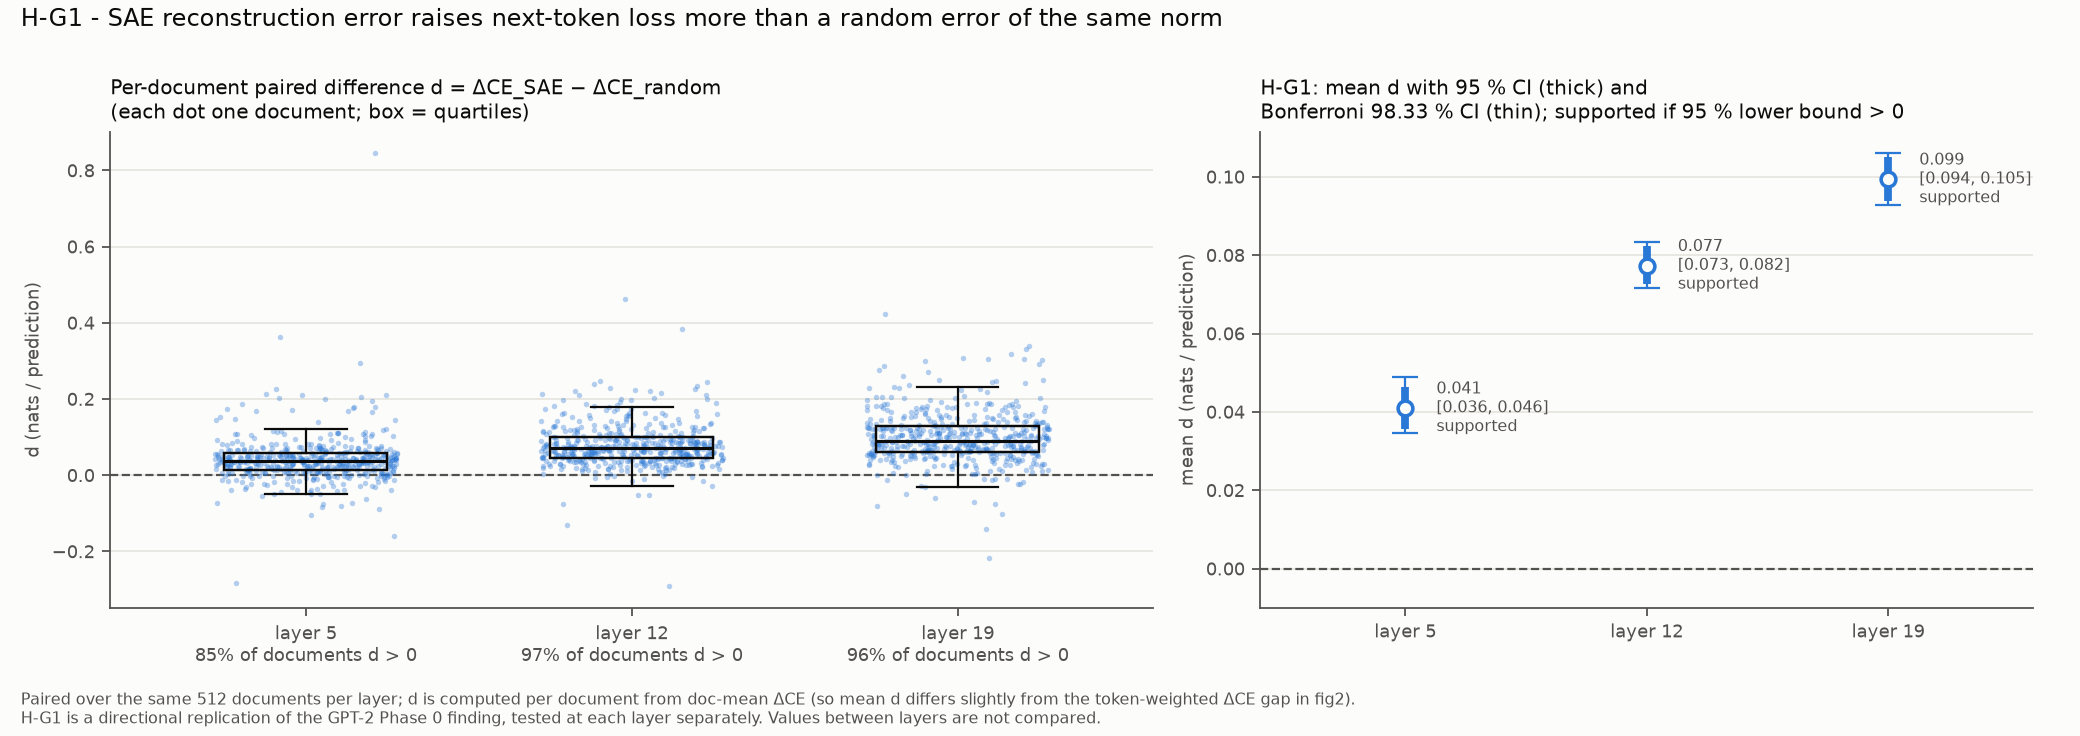
\includegraphics[width=\linewidth]{fig3_h_g1_paired_difference}
  \caption{H-G1 in Gemma-2-2B (\evlabel{validation}). Left: per-document paired difference
  $d=\Delta\mathrm{CE}_{\text{SAE}}-\Delta\mathrm{CE}_{\text{random}}$ (each dot is one of 512 Pile validation documents;
  boxes show quartiles). Right: mean $d$ with 95\,\% (thick) and Bonferroni 98.33\,\% (thin) document-bootstrap
  intervals. Each layer has a different Gemma Scope SAE, so values are not compared between layers. Source:
  \texttt{results/\allowbreak{}gemma2\_pile/\allowbreak{}gemma\_scope\_splicing/\allowbreak{}h\_g1.csv}.}
  \label{fig:m6-hg1}
\end{figure}
